По характерным линиям ртути проверим соответствие градуировки монохроматора. В пределах погрешности характерные линии совпадают с табличными значениями.

Для CdS и CdSe измерим спектральную зависимость фототока
(см. таблицу 1, приложение). Также фитируем зависимость $\lambda(\varphi)$ для монохроматора и нормировку по интенсивности кубическими полиномами. 

С помощью полученных зависимостей найдём отнормированную зависимость фототока $I(\lambda)$, значения и погршеность также см. в таблице 1. Погрешность $\varphi$ -- угла монохроматора, примем равной $10$. Погрешность показаний вольтметра $U$ примем за 2 мВ. 


Построим полученные спектры с учетом нормировки по зависимости эффективности монохроматора от длины волны. Графики приведены на рис. \ref{fig:spec}.

\begin{figure}[h]
    \centering
    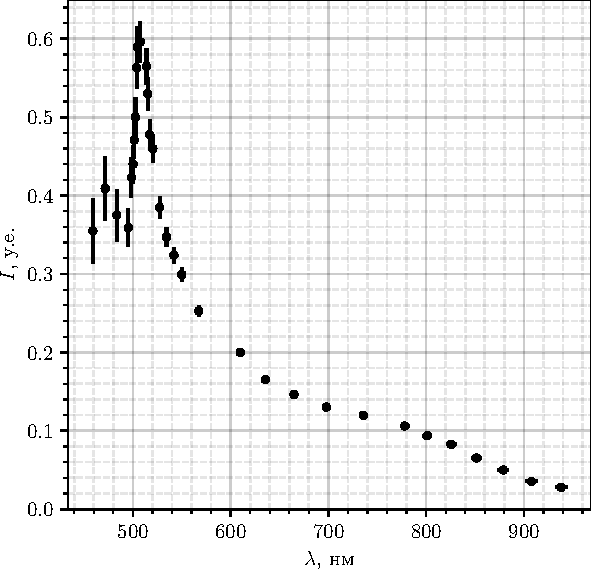
\includegraphics[width=0.45\textwidth]{plot_CdS_6.11.2.pdf}
    \hspace{5 mm} 
    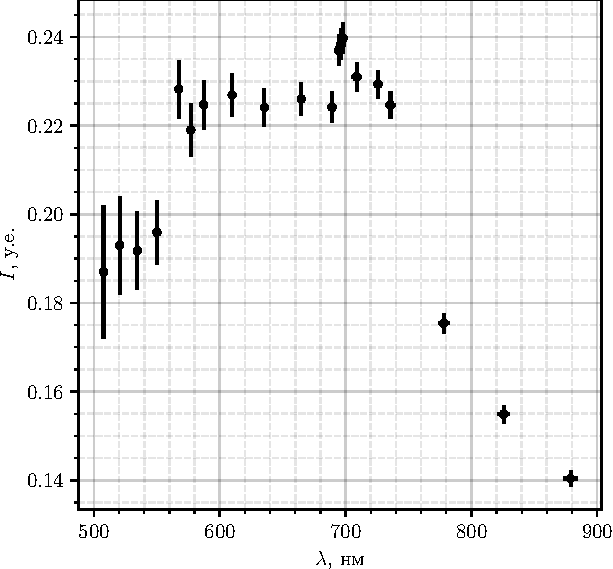
\includegraphics[width=0.45\textwidth]{plot_CdSe_6.11.2.pdf}
    \caption{Спектральная зависимость фототока для CdS (сера) и CdSe (селен)}
    \label{fig:spec}
\end{figure}

В образце с серой можем оценить красную границу $\sub{\lambda}{S}^{\text{кр}} = 570$ нм, тогда $\sub{E}{S}^{\text{эксп}} = 2.2$ эВ, что достаточно близко к табличному значению $\sub{E}{S}^{\text{табл}} = 2.42$ эВ. Также можем наблюдать примесный пик (излом) в районе $800$ нм, что соответствует $1.6$ эВ. 



В образце с селеном можем оценить красную границу $\sub{\lambda}{Se}^{\text{кр}} = 750$ нм, тогда $\sub{E}{Se}^{\text{эксп}} = 1.7$ эВ, что достаточно совпадает с табличным значением $\sub{E}{Se}^{\text{табл}} = 1.74$ эВ. Также можем наблюдать плато в районе $650$ нм, что соответствует $1.9$ эВ. 




\subsection*{Вывод}

Исследована собственная фотопроводимость полупроводников (CdS и CdSe). По полученным спектральным зависимостям фототока определены ширины запрещенных зон. Получены значения совпадающие с табличными в пределах погрешности, обусловленной формальностью графического определения красной границы фотопроводимости. Наблюдались примеси в SdS.